\documentclass[a4paper,14pt]{article}
\usepackage[utf8]{inputenc}  %% 1
\usepackage[T2A]{fontenc}      %% 2
\usepackage[english,russian]{babel}    %% 3
\usepackage{amssymb, amsmath,mathtext,cite,enumerate,float}
\usepackage{helvet}
\usepackage{matlab-prettifier}
\usepackage{graphicx}

\parindent=1.25cm

\newcommand*{\No}{\textnumero}

\begin{document}

\begin{titlepage}
\newpage

\begin{center}
Санкт-Петербургский государственный политехнический университет \\
\end{center}

\begin{center}
Институт прикладной математики и механики \\ 
\end{center}

\begin{center}
\textbf{Кафедра "Прикладная математика и информатика"} \\ 
\end{center}

\vspace{2em}

\begin{center}
\LARGE{\textbf{Отчет по лабоработрной работе 1}}
\end{center}

\vspace{14em}


\begin{center}
Санкт-Петербург \\2018
\end{center}

\end{titlepage}

\section{Постановка задачи}
Ознакомиться с пакетными реализациями метода опорных векторов. Протестировать их на различных наборах данных, проанализировав зависимость результатов от подбора гиперпараметров.

\section{Используемые функции}

В данной работе использовалась реализация метода опорных векторов из пакета scikit-learn для языка Python. Пример использования приведен в листинге \ref{lst:usage}

\begin{lstlisting}[caption={Использование svm из пакета scikit-learn}, label={lst:usage}, language=Python]
import sklearn.svm as svm
gnb = clf = svm.SVC()
y_pred = gnb.fit(x, y).predict(x)
\end{lstlisting}

\textbf{Аргументы и возвращаемые значения:}
\begin{itemize}
	\item функции fit(x, y):\\ {[in]} x - матрица данных; {[in]} y - вектор меток классов. {[out]} экземпляр классификатора, обученный на соответсвующих данных
	\item функции predict(x): \\ {[in]} x - матрица данных. {[out]} возвращает вектор предсказанных меток.
\end{itemize}

\section{Проделанная работа}

\subsection{Задание 1}

\textbf{Постановка задачи:}

Постройте алгоритм метода опорных векторов типа "C-classification" с параметром C = 1, используя ядро "linear". Визуализируйте разбиение пространства признаков на области с помощью полученной модели. Выведите количество полученных опорных векторов, а также ошибки классификации на обучающей и тестовой выборках.

Иллюстрации и результаты вычислений приведены на рис. \ref{graph:task_1c1}-\ref{graph:task_5c1}

\begin{figure}[H]
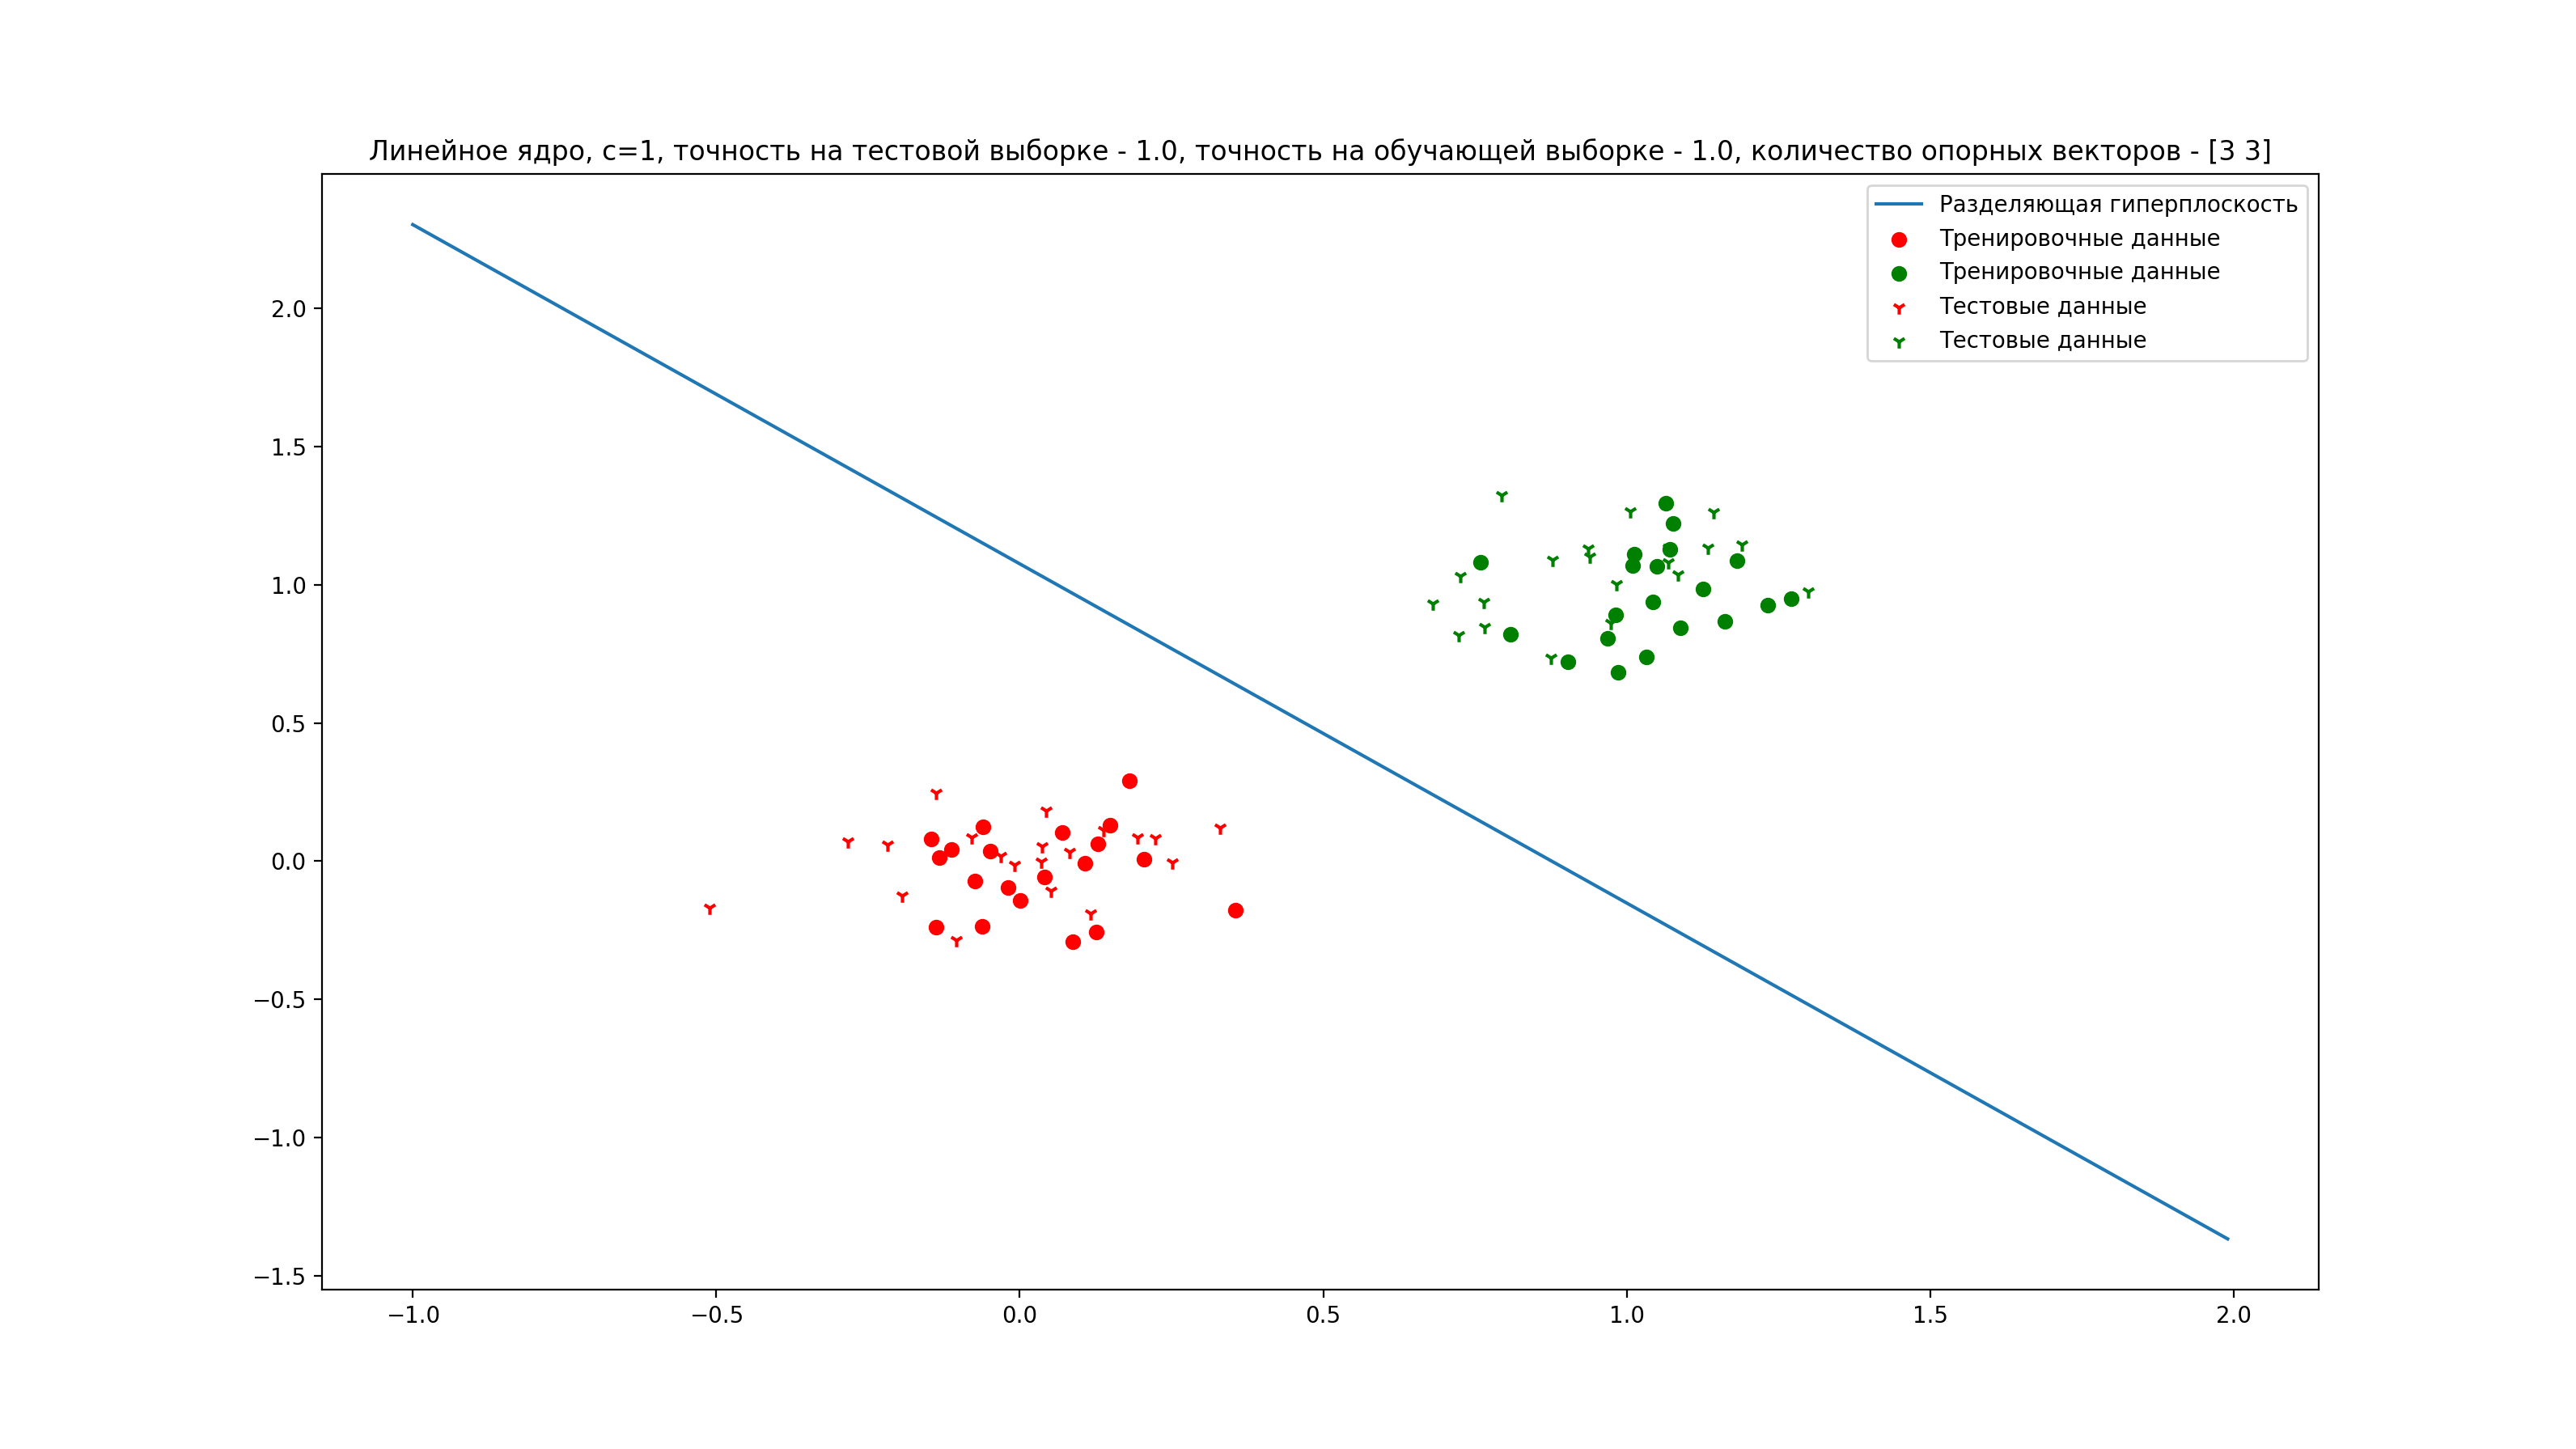
\includegraphics[width=\textwidth, keepaspectratio]{task_1c1.png}
\caption{SVM для датасета 1}
\label{graph:task_1c1}
\end{figure}


\begin{figure}[H]
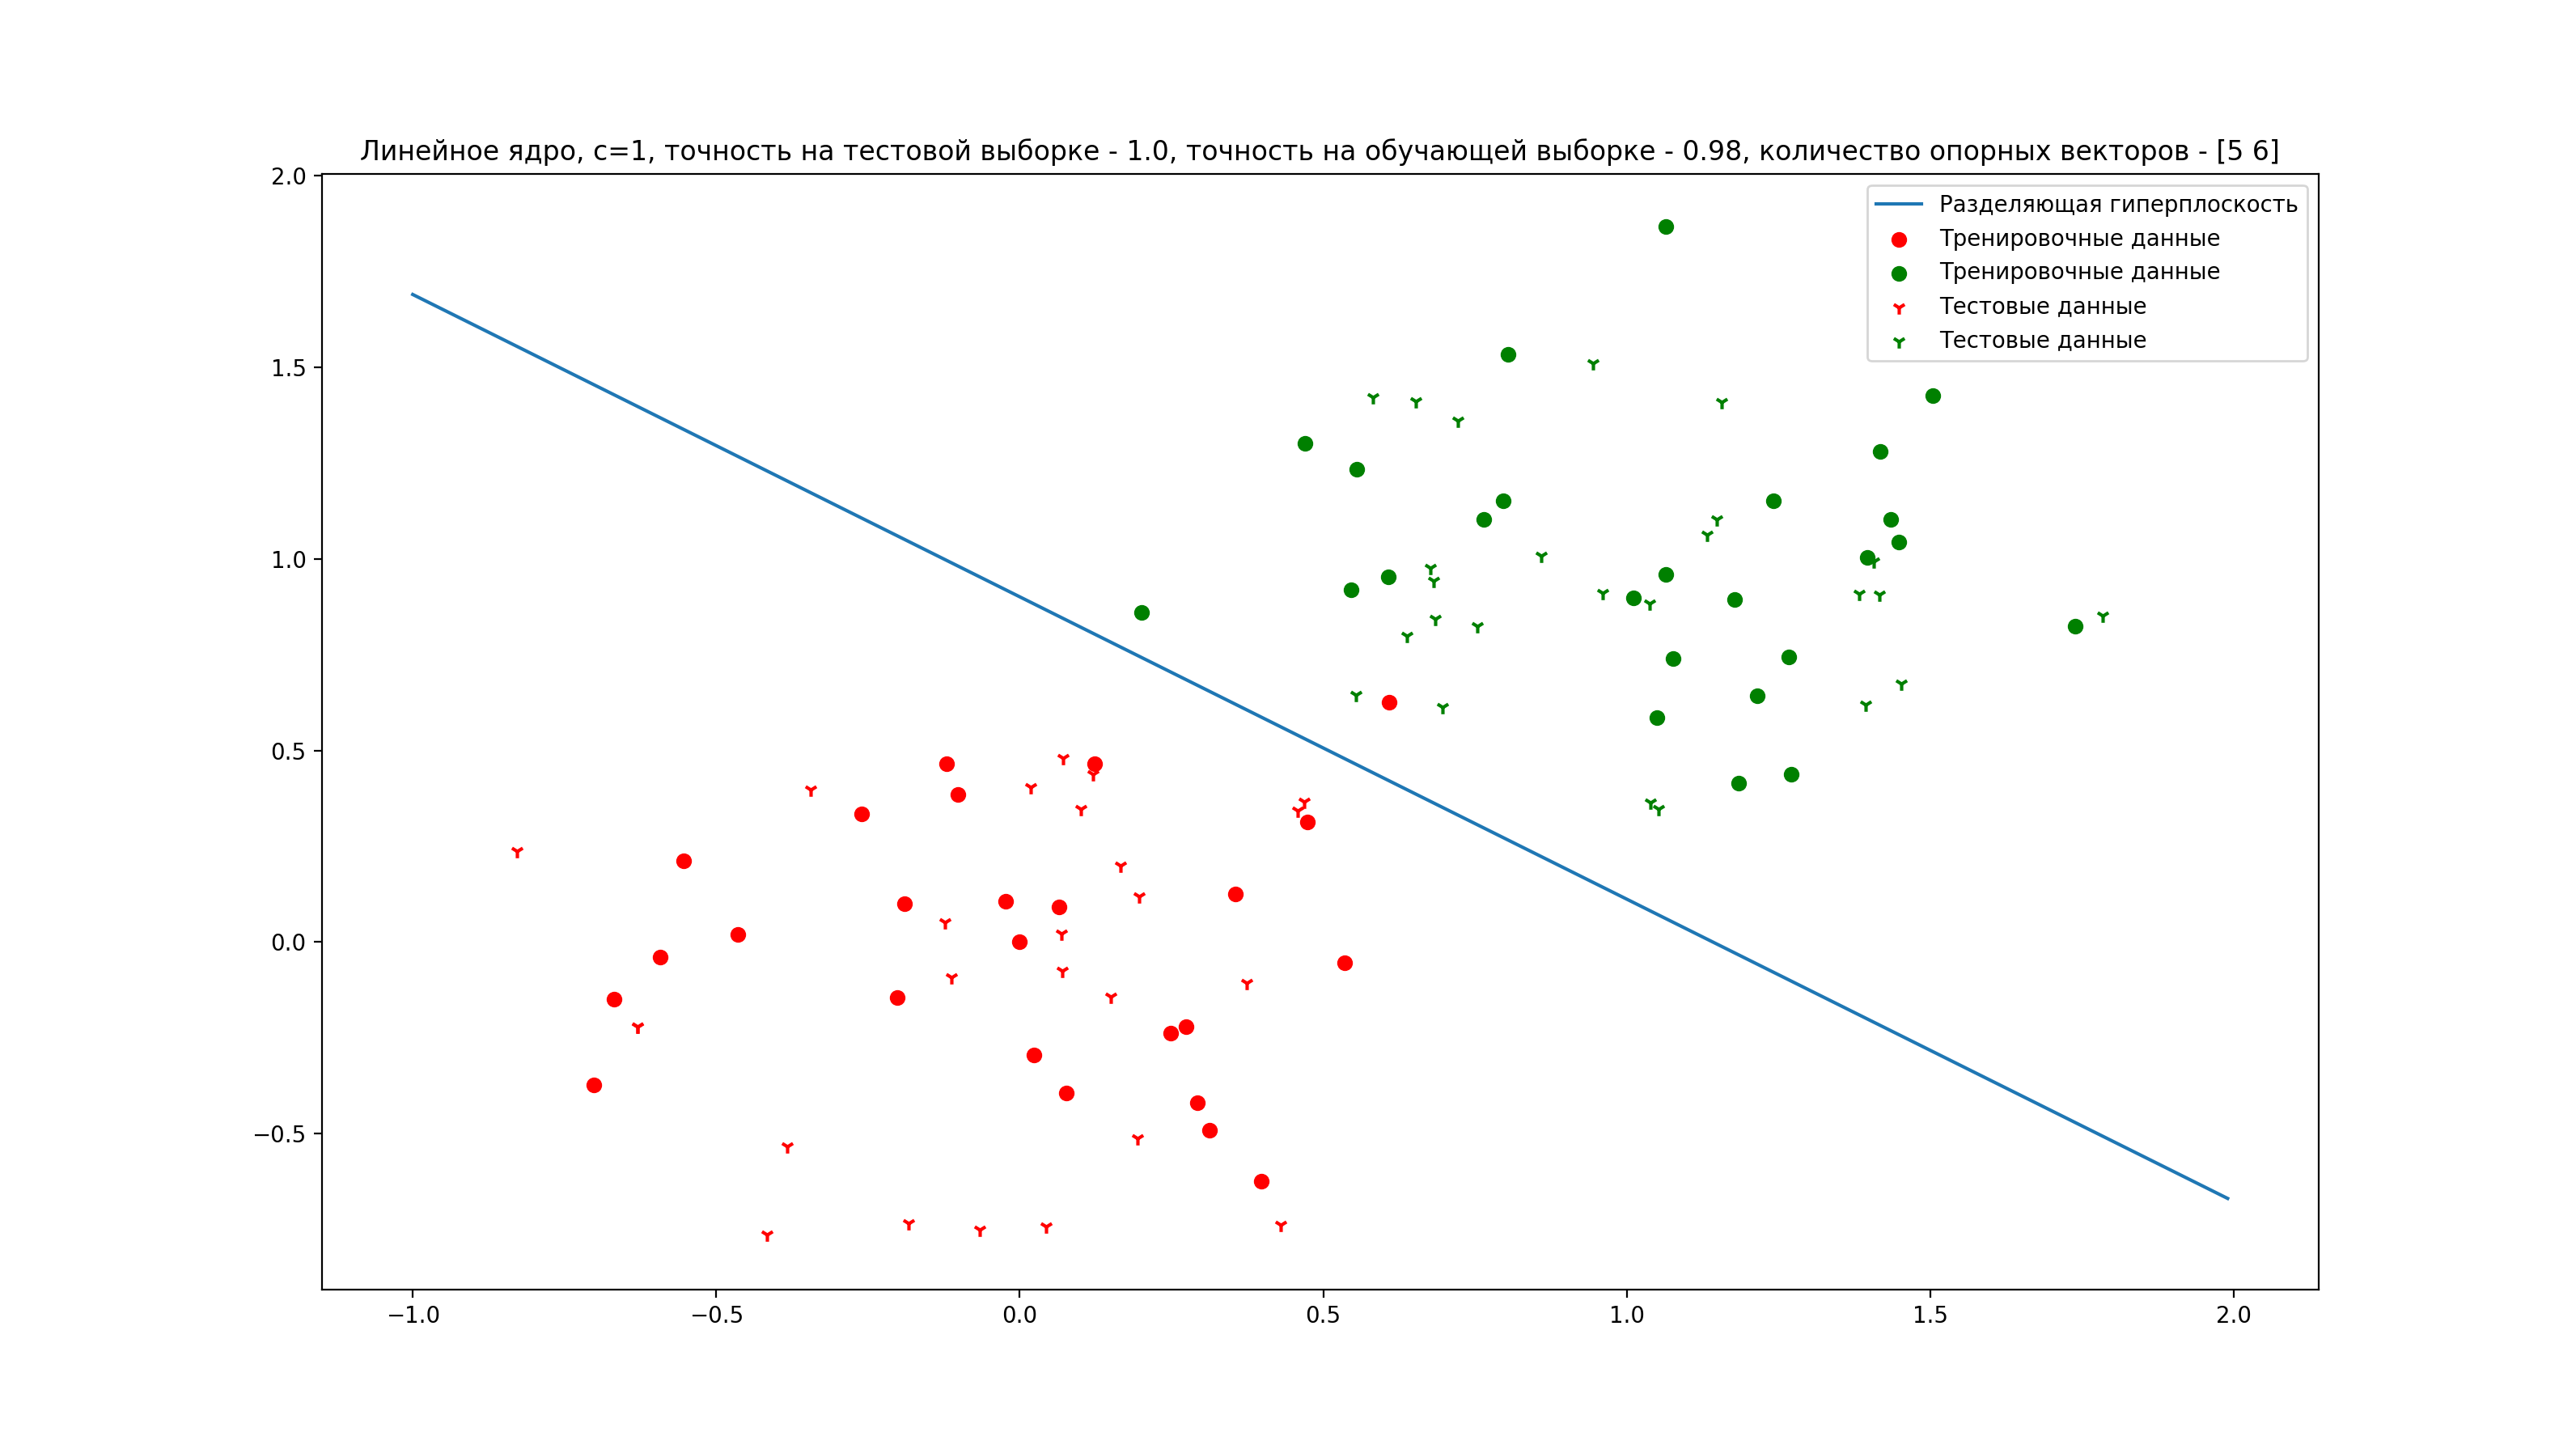
\includegraphics[width=\textwidth, keepaspectratio]{task_2c1.png}
\caption{SVM для датасета 2}
\label{graph:task_2c1}
\end{figure}

\begin{figure}[H]
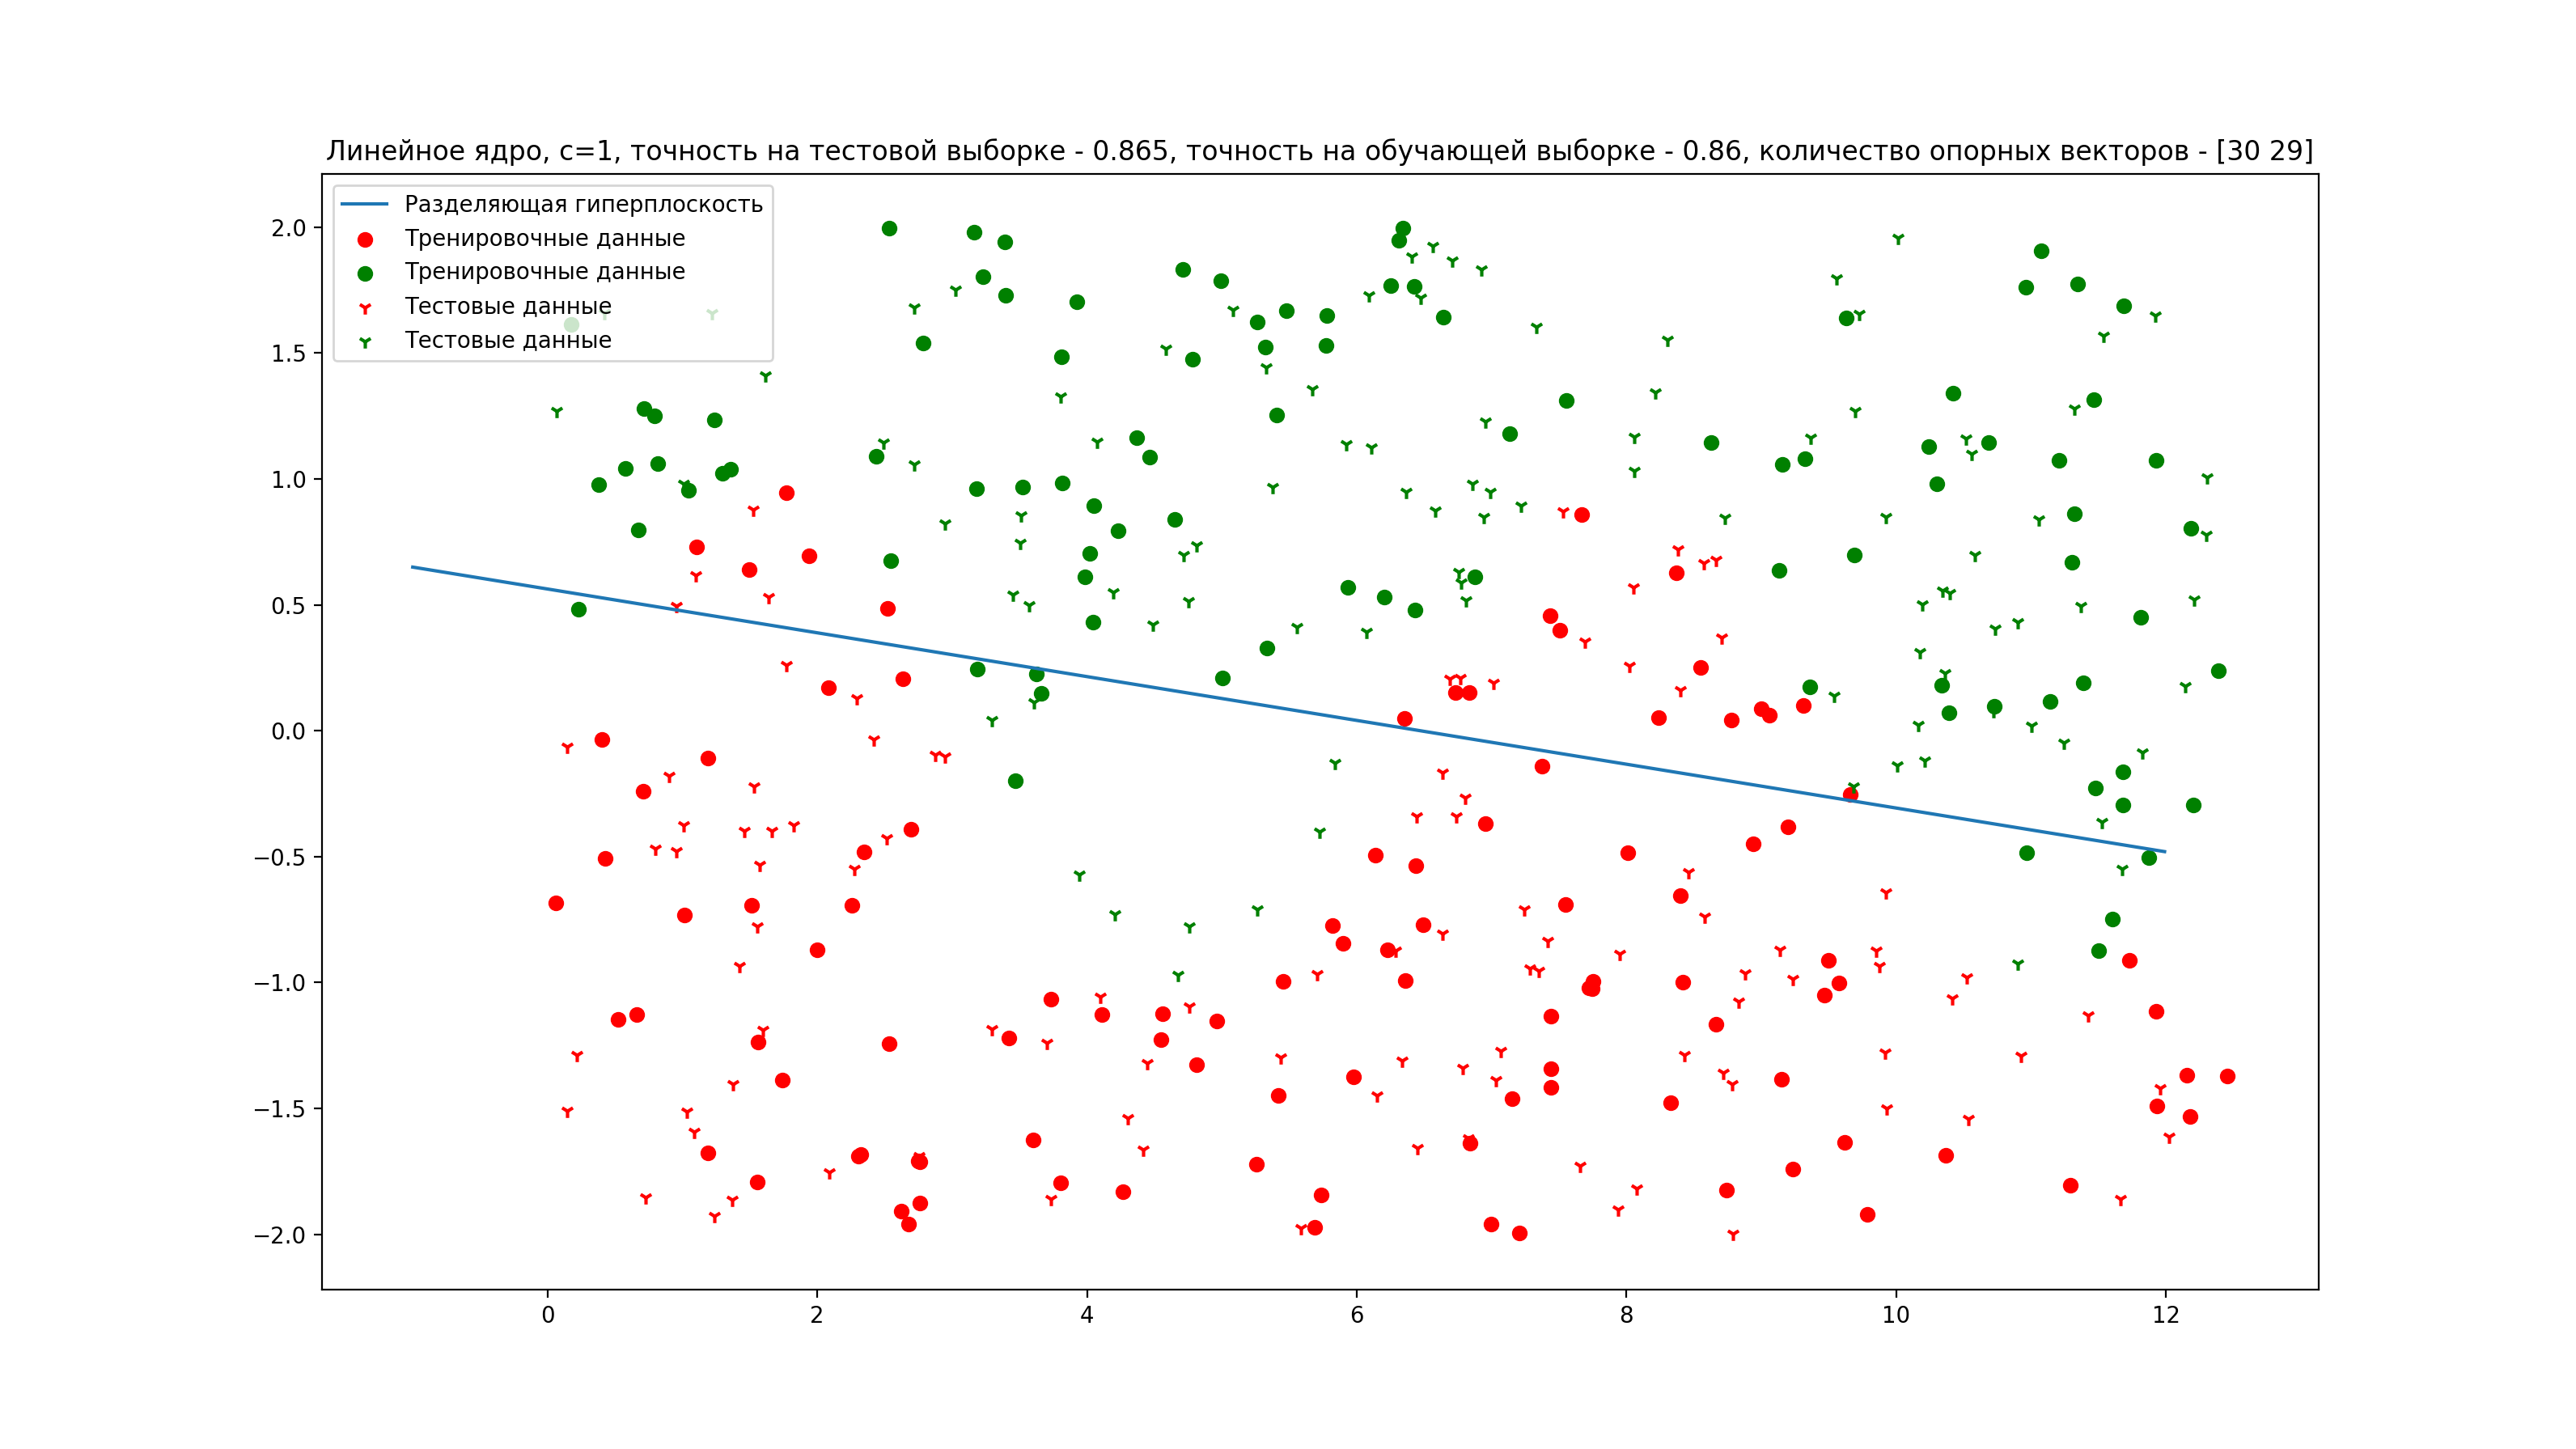
\includegraphics[width=\textwidth, keepaspectratio]{task_4c1.png}
\caption{SVM для датасета 4}
\label{graph:task_4c1}
\end{figure}

\begin{figure}[H]
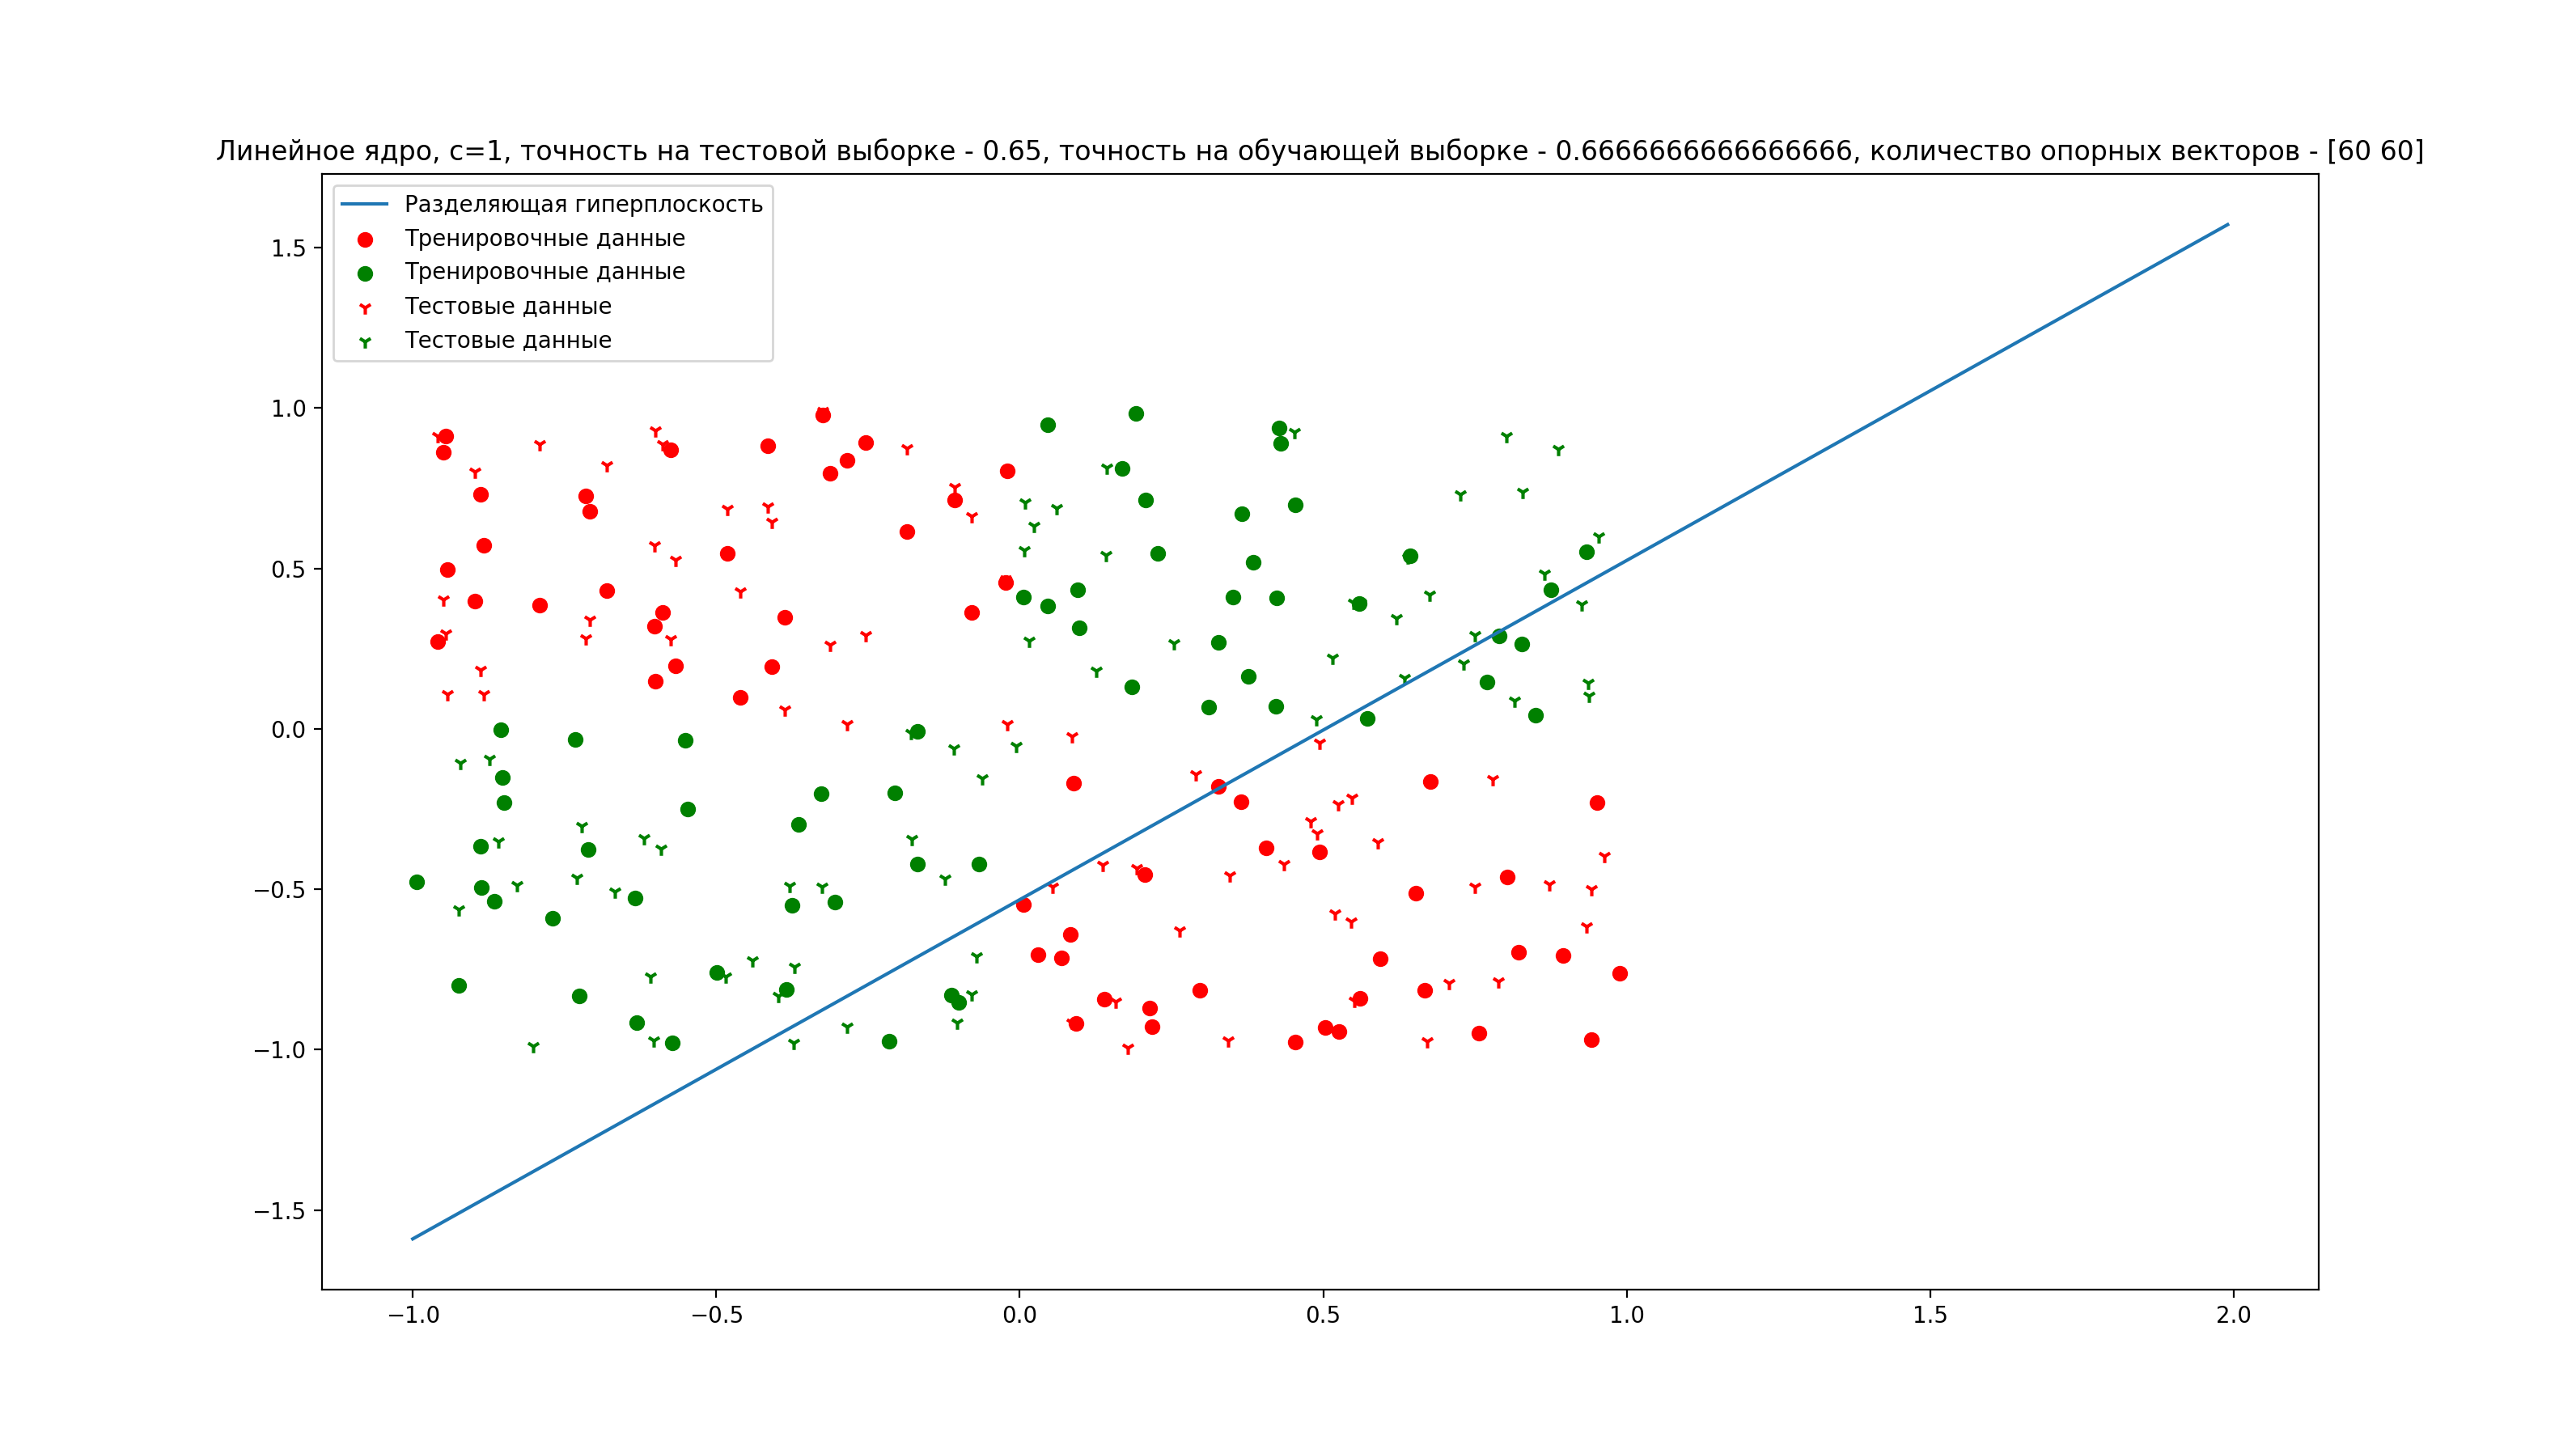
\includegraphics[width=\textwidth, keepaspectratio]{task_5c1.png}
\caption{SVM для датасета 5}
\label{graph:task_5c1}
\end{figure}

Из приведенных рисунков видно, что линейное ядро показывает плохие результаты в случаях, когда классы не являются линейно разделимыми (что абсолютно логично). Так же стоит отметить, что чем сложнее отделимы классы, тем больше опорных векторов приходится включать в систему.

\subsection{Задание 2}

\textbf{Постановка задачи:}
Используя алгоритм метода опорных векторов типа "C-classification" с линейным ядром, добейтесь нулевой ошибки сначала на обучающей выборке, а затем на тестовой, путем изменения параметра C. Выберите оптимальное значение данного параметра и объясните свой выбор. Всегда ли нужно добиваться минимизации ошибки на обучающей выборке?

Попробуем добиться точности 1 на обучающей выборке для датасета 2. Информация о конфигурации системы в этом случае приведена на рис. \ref{graph:task_2_train_acc}. Как видно из результатов, увеличение параметра С, отвечающего за вес ошибки на обучающей выборке, помогло добиться желаемого, однако, в данном случае это привело к переобучению: точность на тестовой выборке упала.

На остальных датасетах нужной точности добиться невозможно в силу невозможности линейного разделения данных. 

\begin{figure}[H]
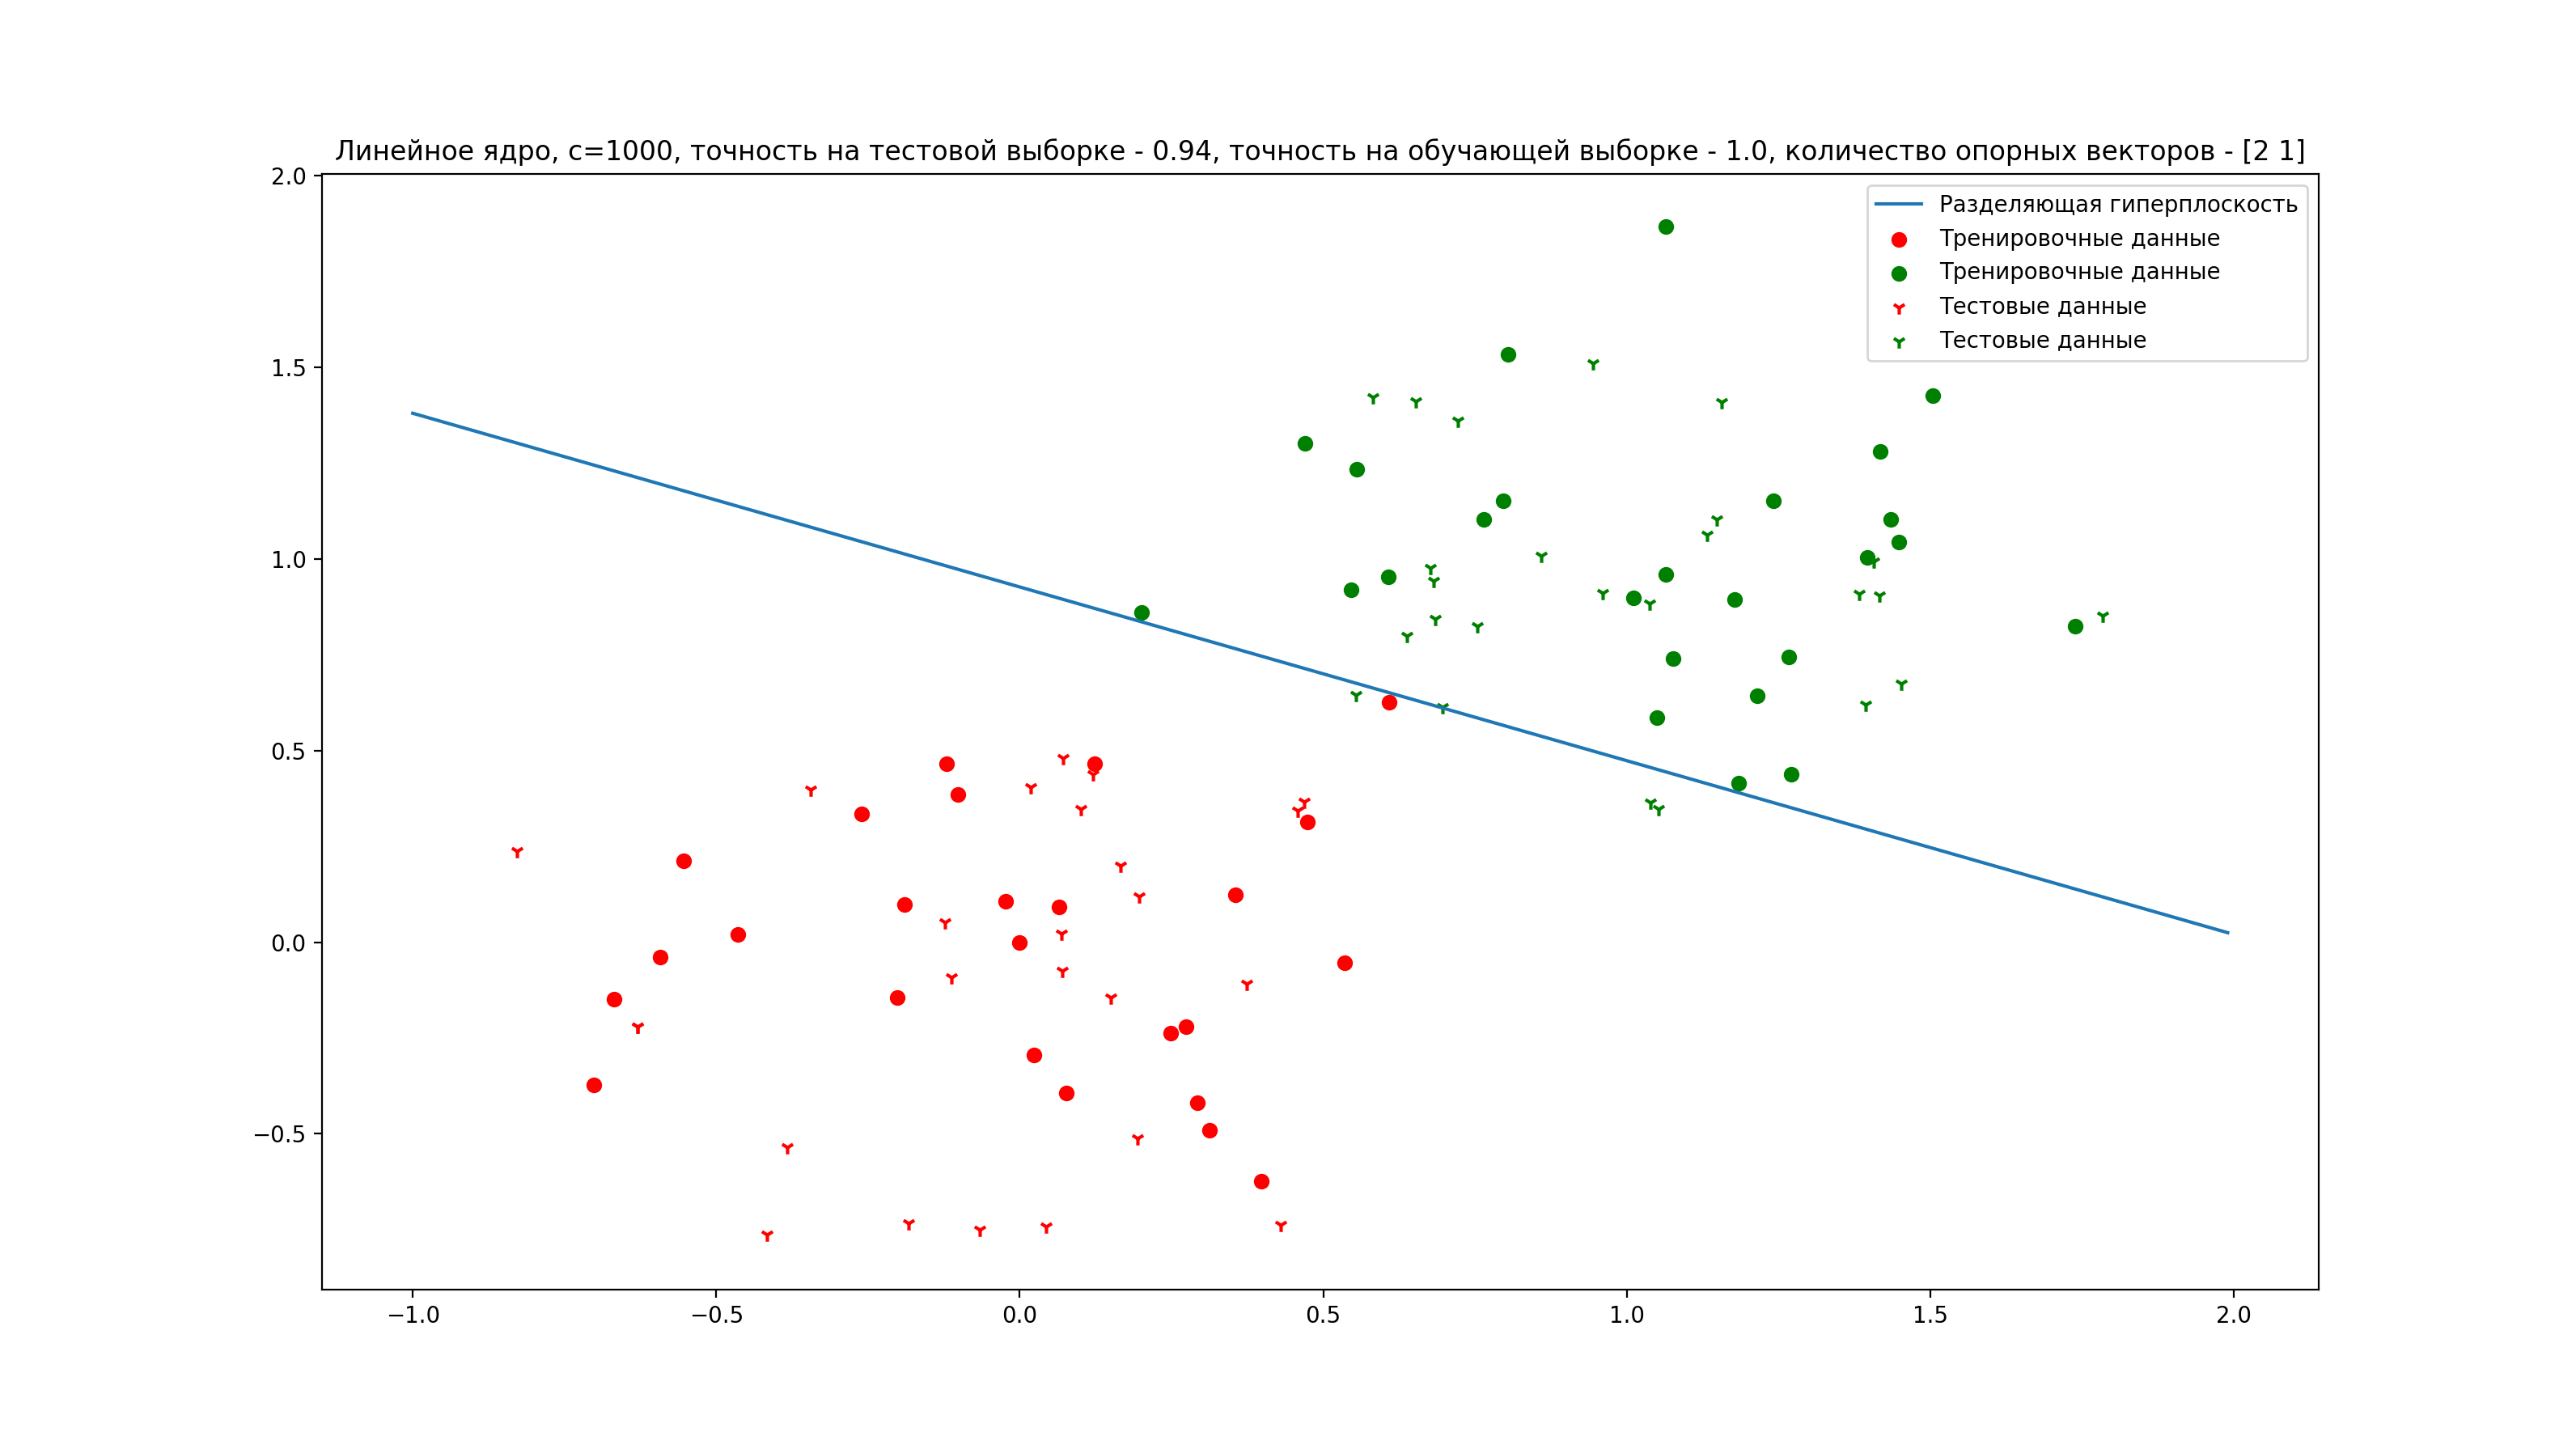
\includegraphics[width=\textwidth, keepaspectratio]{task_2c1000.png}
\caption{SVM для датасета 5}
\label{graph:task_2_train_acc}
\end{figure}

\subsection{Задания 3, 4}

Среди ядер <<polynomial>>, <<radial>> и <<sigmoid>> выберите оптимальное в плане количества ошибок на тестовой выборке. Попробуйте различные значения параметра degree для полиномиального ядра.

Среди ядер <<polynomial>>, <<radial>> и <<sigmoid>> выберите оптимальное в плане количества ошибок на тестовой выборке.

\begin{figure}[H]
\resizebox{\columnwidth}{!}
{
\begin{tabular}{l l l l}
Номер датасета & Тип ядра & Точность на тренировочной выборке & Точность на тестовой выборке\\
2 & rbf & 0.98 & 0.96 \\
 & sigmoid & 0.97 & 0.98  \\
 & poly (deg = 2) & 0.97 & 0.98 \\
 & poly (deg = 3) & 0.96 & 0.98 \\
 & poly (deg = 4) & 0.95 & 0.94 \\
 & poly (deg = 5) & 0.94 & 0.94 \\
4 & rbf & 0.97 & 0.95 \\
 & sigmoid & 0.52 & 0.55 \\
 & poly (deg = 2) & 0.84 & 0.83 \\
 & poly (deg = 3) & 0.87 & 0.87 \\
5 & rbf & 0.91 & 0.79 \\
 & sigmoid & 0.67 & 0.25 \\
 & poly (deg = 2) & 0.91 & 0.88 \\
 & poly (deg = 3) & 0.63 & 0.21 \\
 & poly (deg = 4) & 0.79 & 0.8 \\
 & poly (deg = 5) & 0.57 & 0.49 \\
\end{tabular}
}
\caption{Результаты обучения с разными ядрами}
\label{tbl:kernels}

\end{figure}

\subsection{Задание 5}

\textbf{Постановка задачи:}

Среди ядер <<polynomial>>, <<radial>> и <<sigmoid>> выберите оптимальное в плане количества ошибок на тестовой выборке. Изменяя значение параметра gamma, продемонстрируйте эффект переобучения, выполните при этом визуализацию разбиения пространства признаков на области.

Для каждого датасета рассмотрим наилучшее ядро, выбранное в предыдущем шаге. Зависимость точности обучения от параметра gamma приведена на рис. \ref{graph:task_2_gamma} - \ref{graph:task_5_gamma}.

\begin{figure}[H]
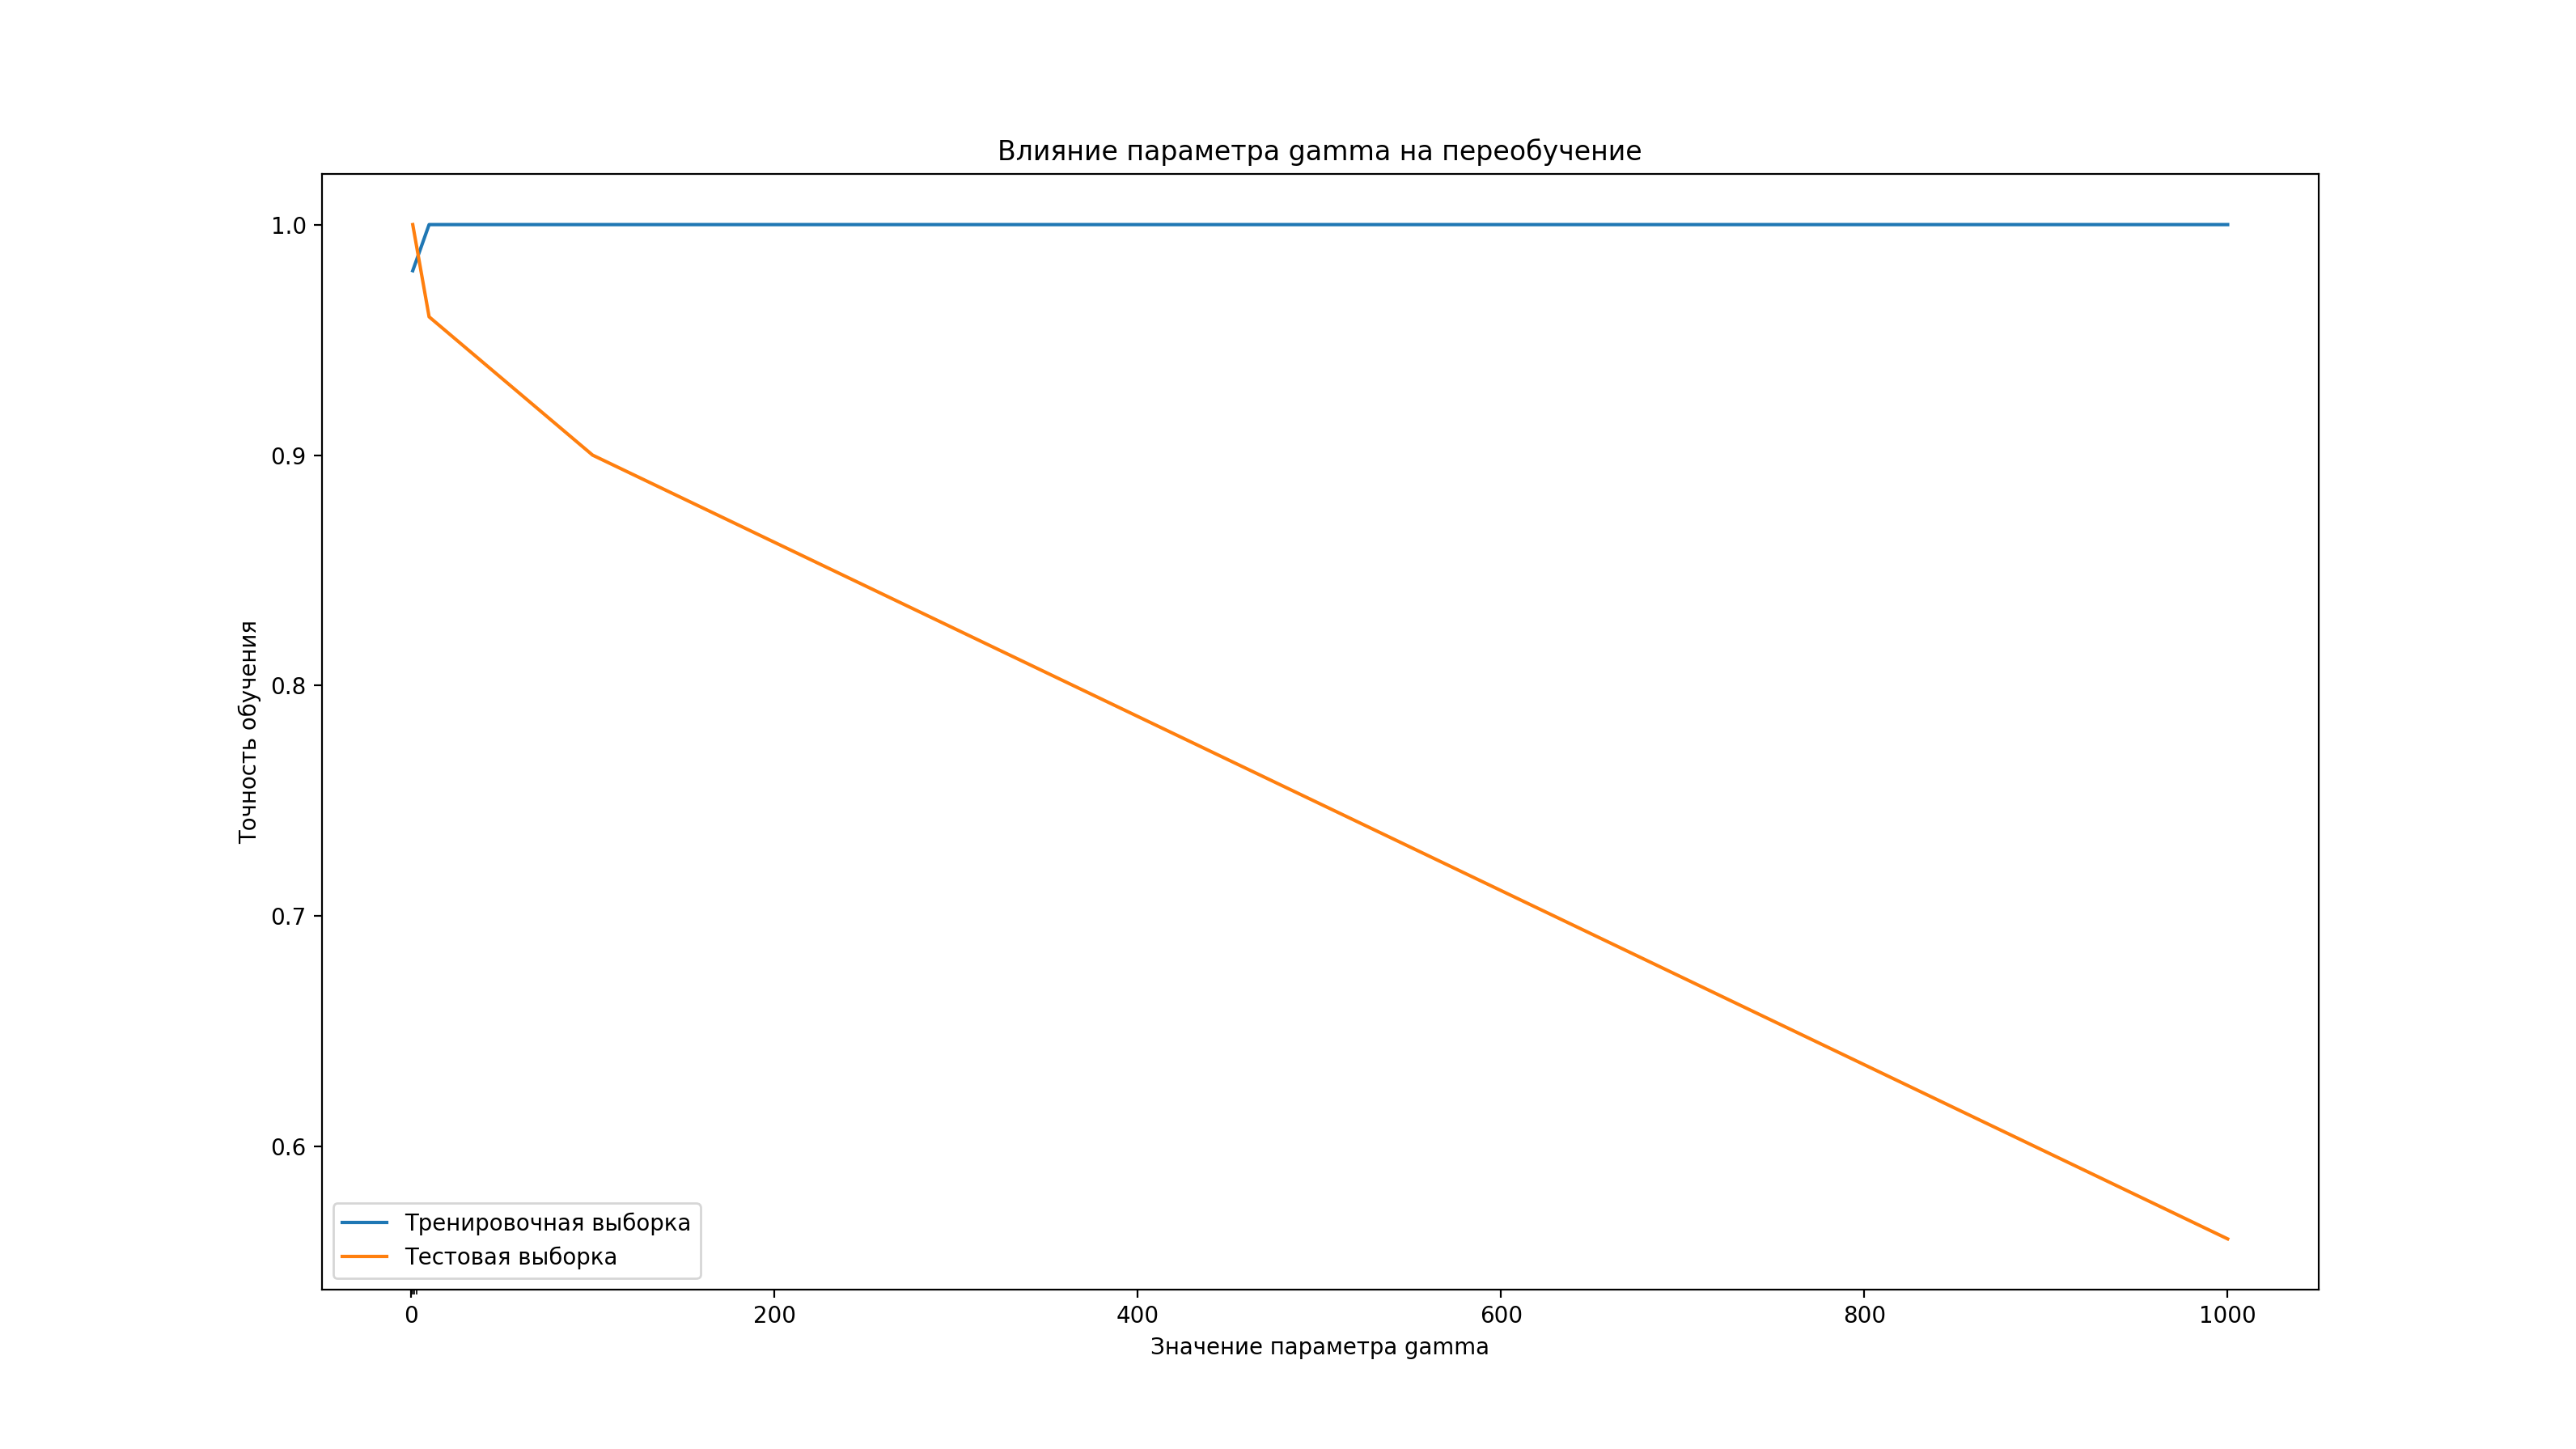
\includegraphics[width=\textwidth, keepaspectratio]{task2_gamma.png}
\caption{Переобучение на датасете 2}
\label{graph:task_2_gamma}
\end{figure}

\begin{figure}[H]
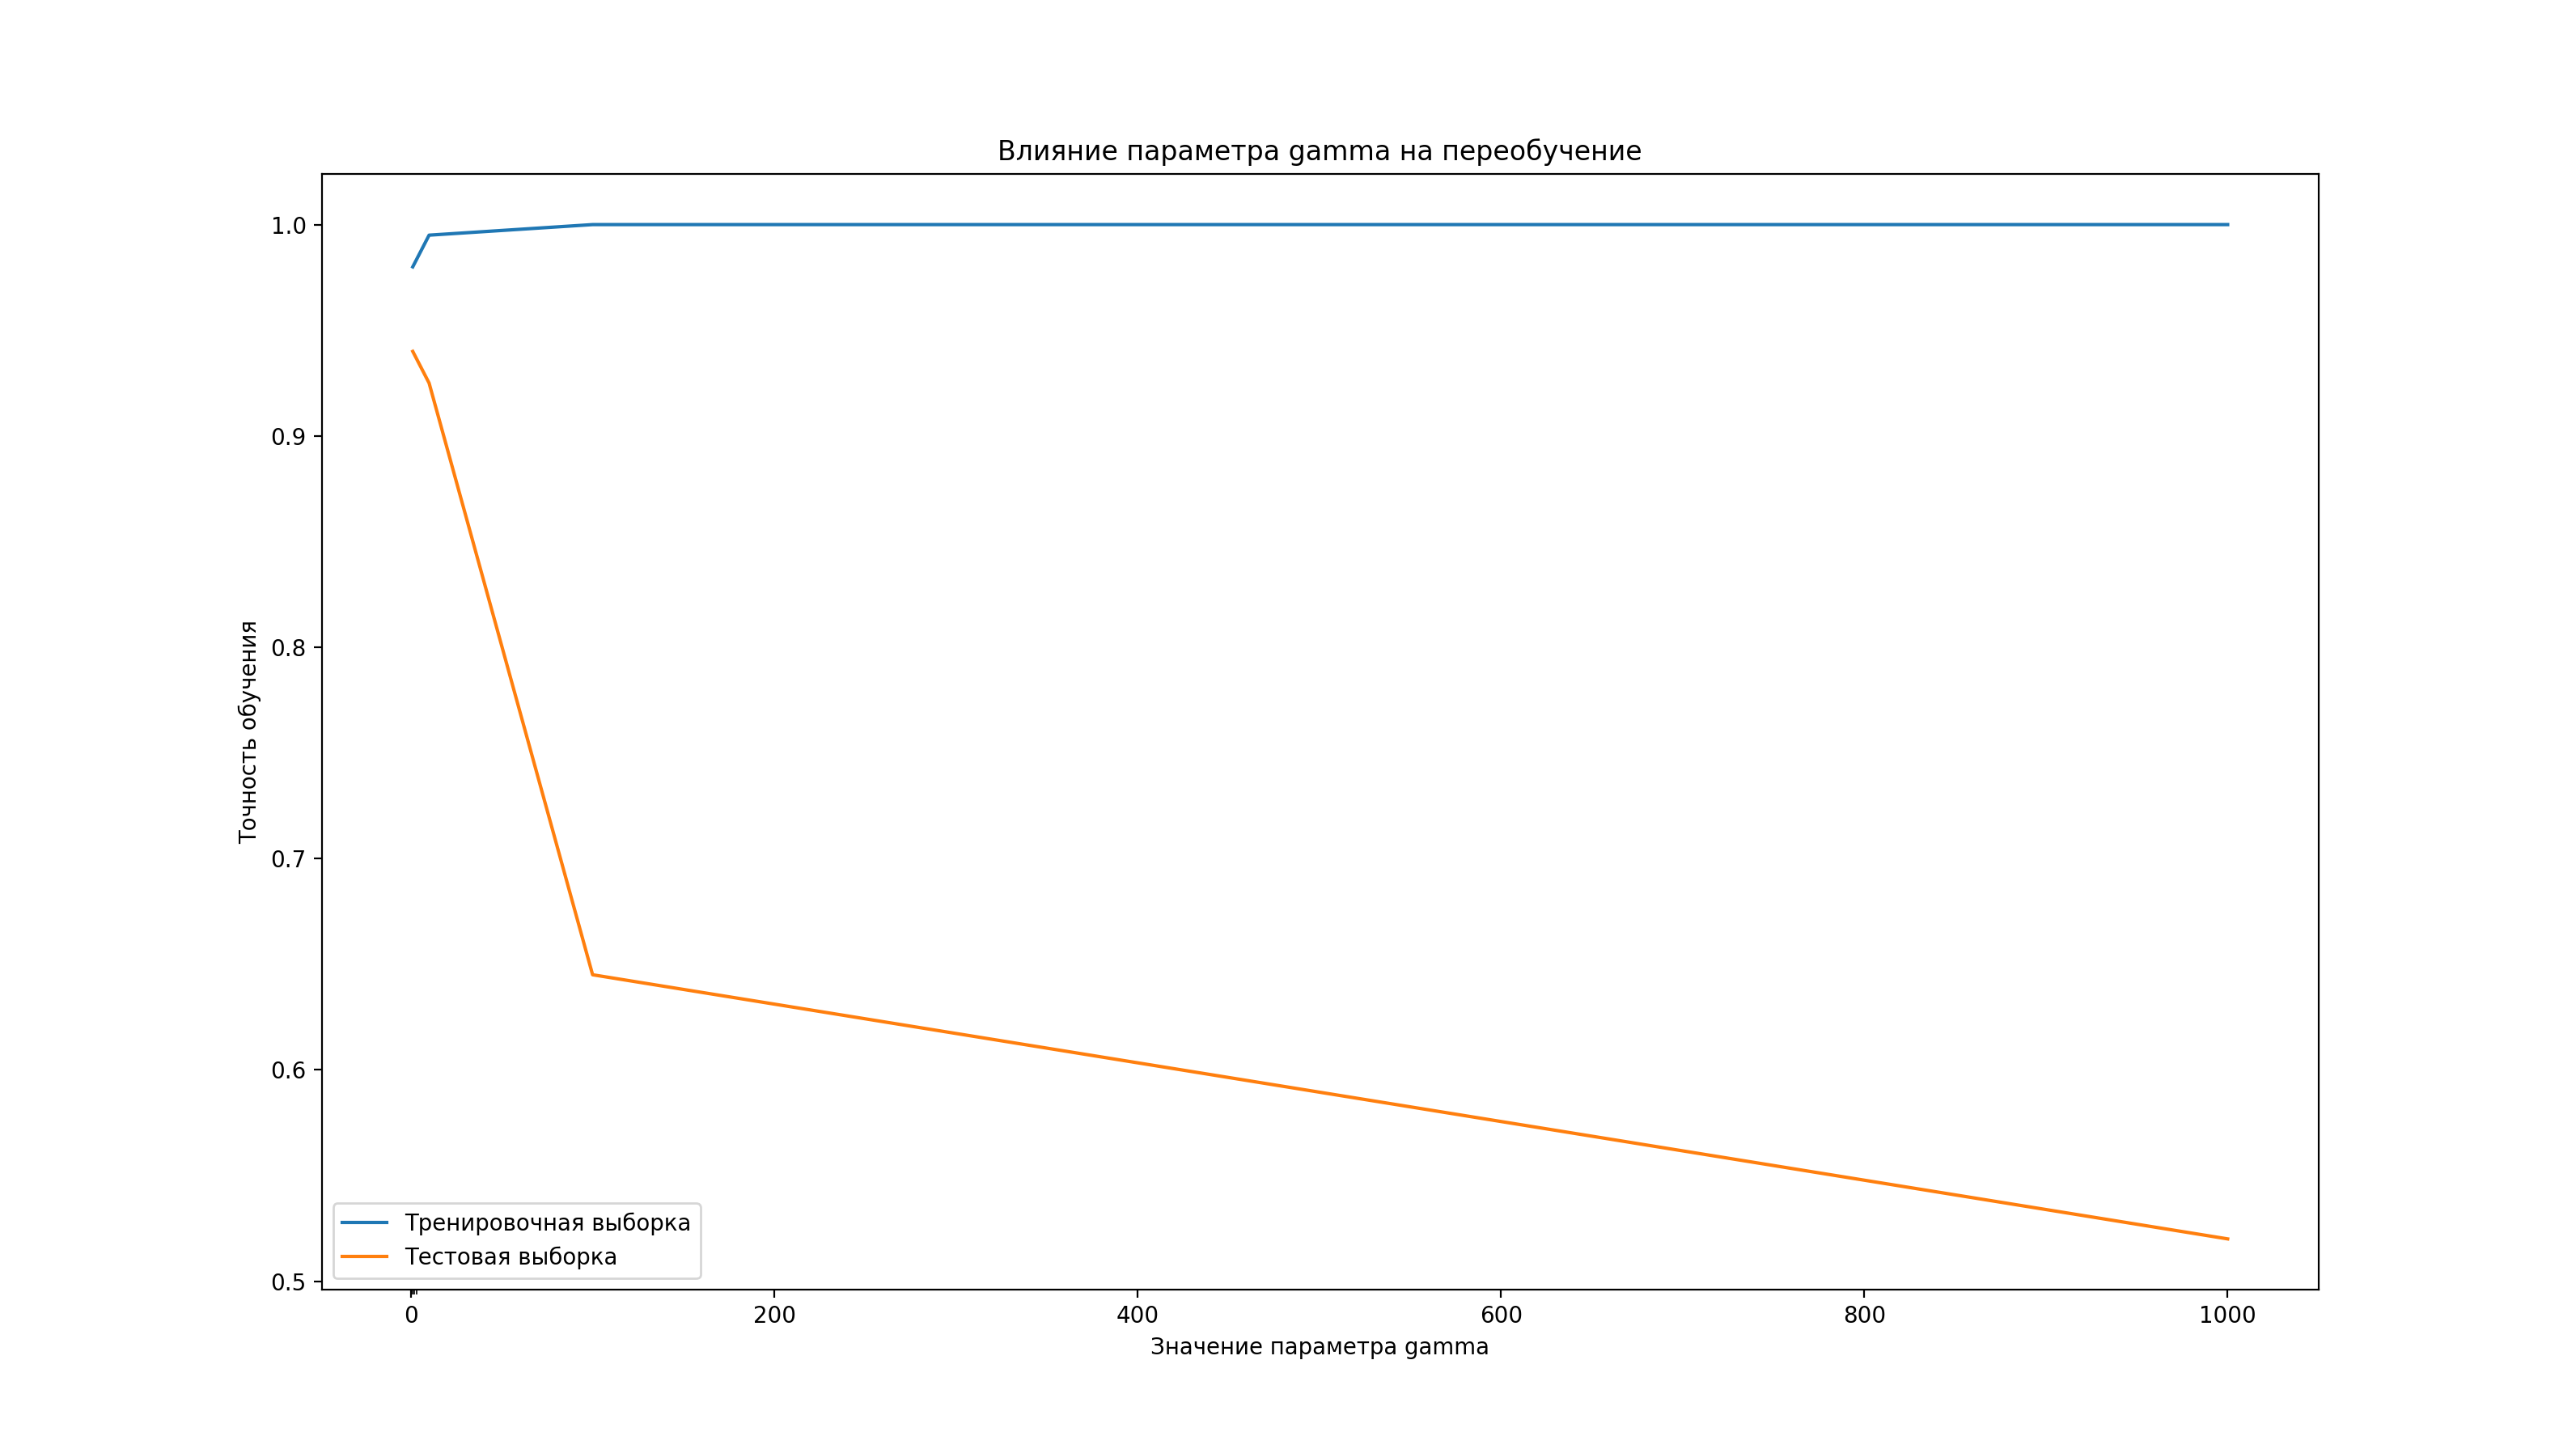
\includegraphics[width=\textwidth, keepaspectratio]{task4_gamma.png}
\caption{Переобучение на датасете 4}
\label{graph:task_4_gamma}
\end{figure}

\begin{figure}[H]
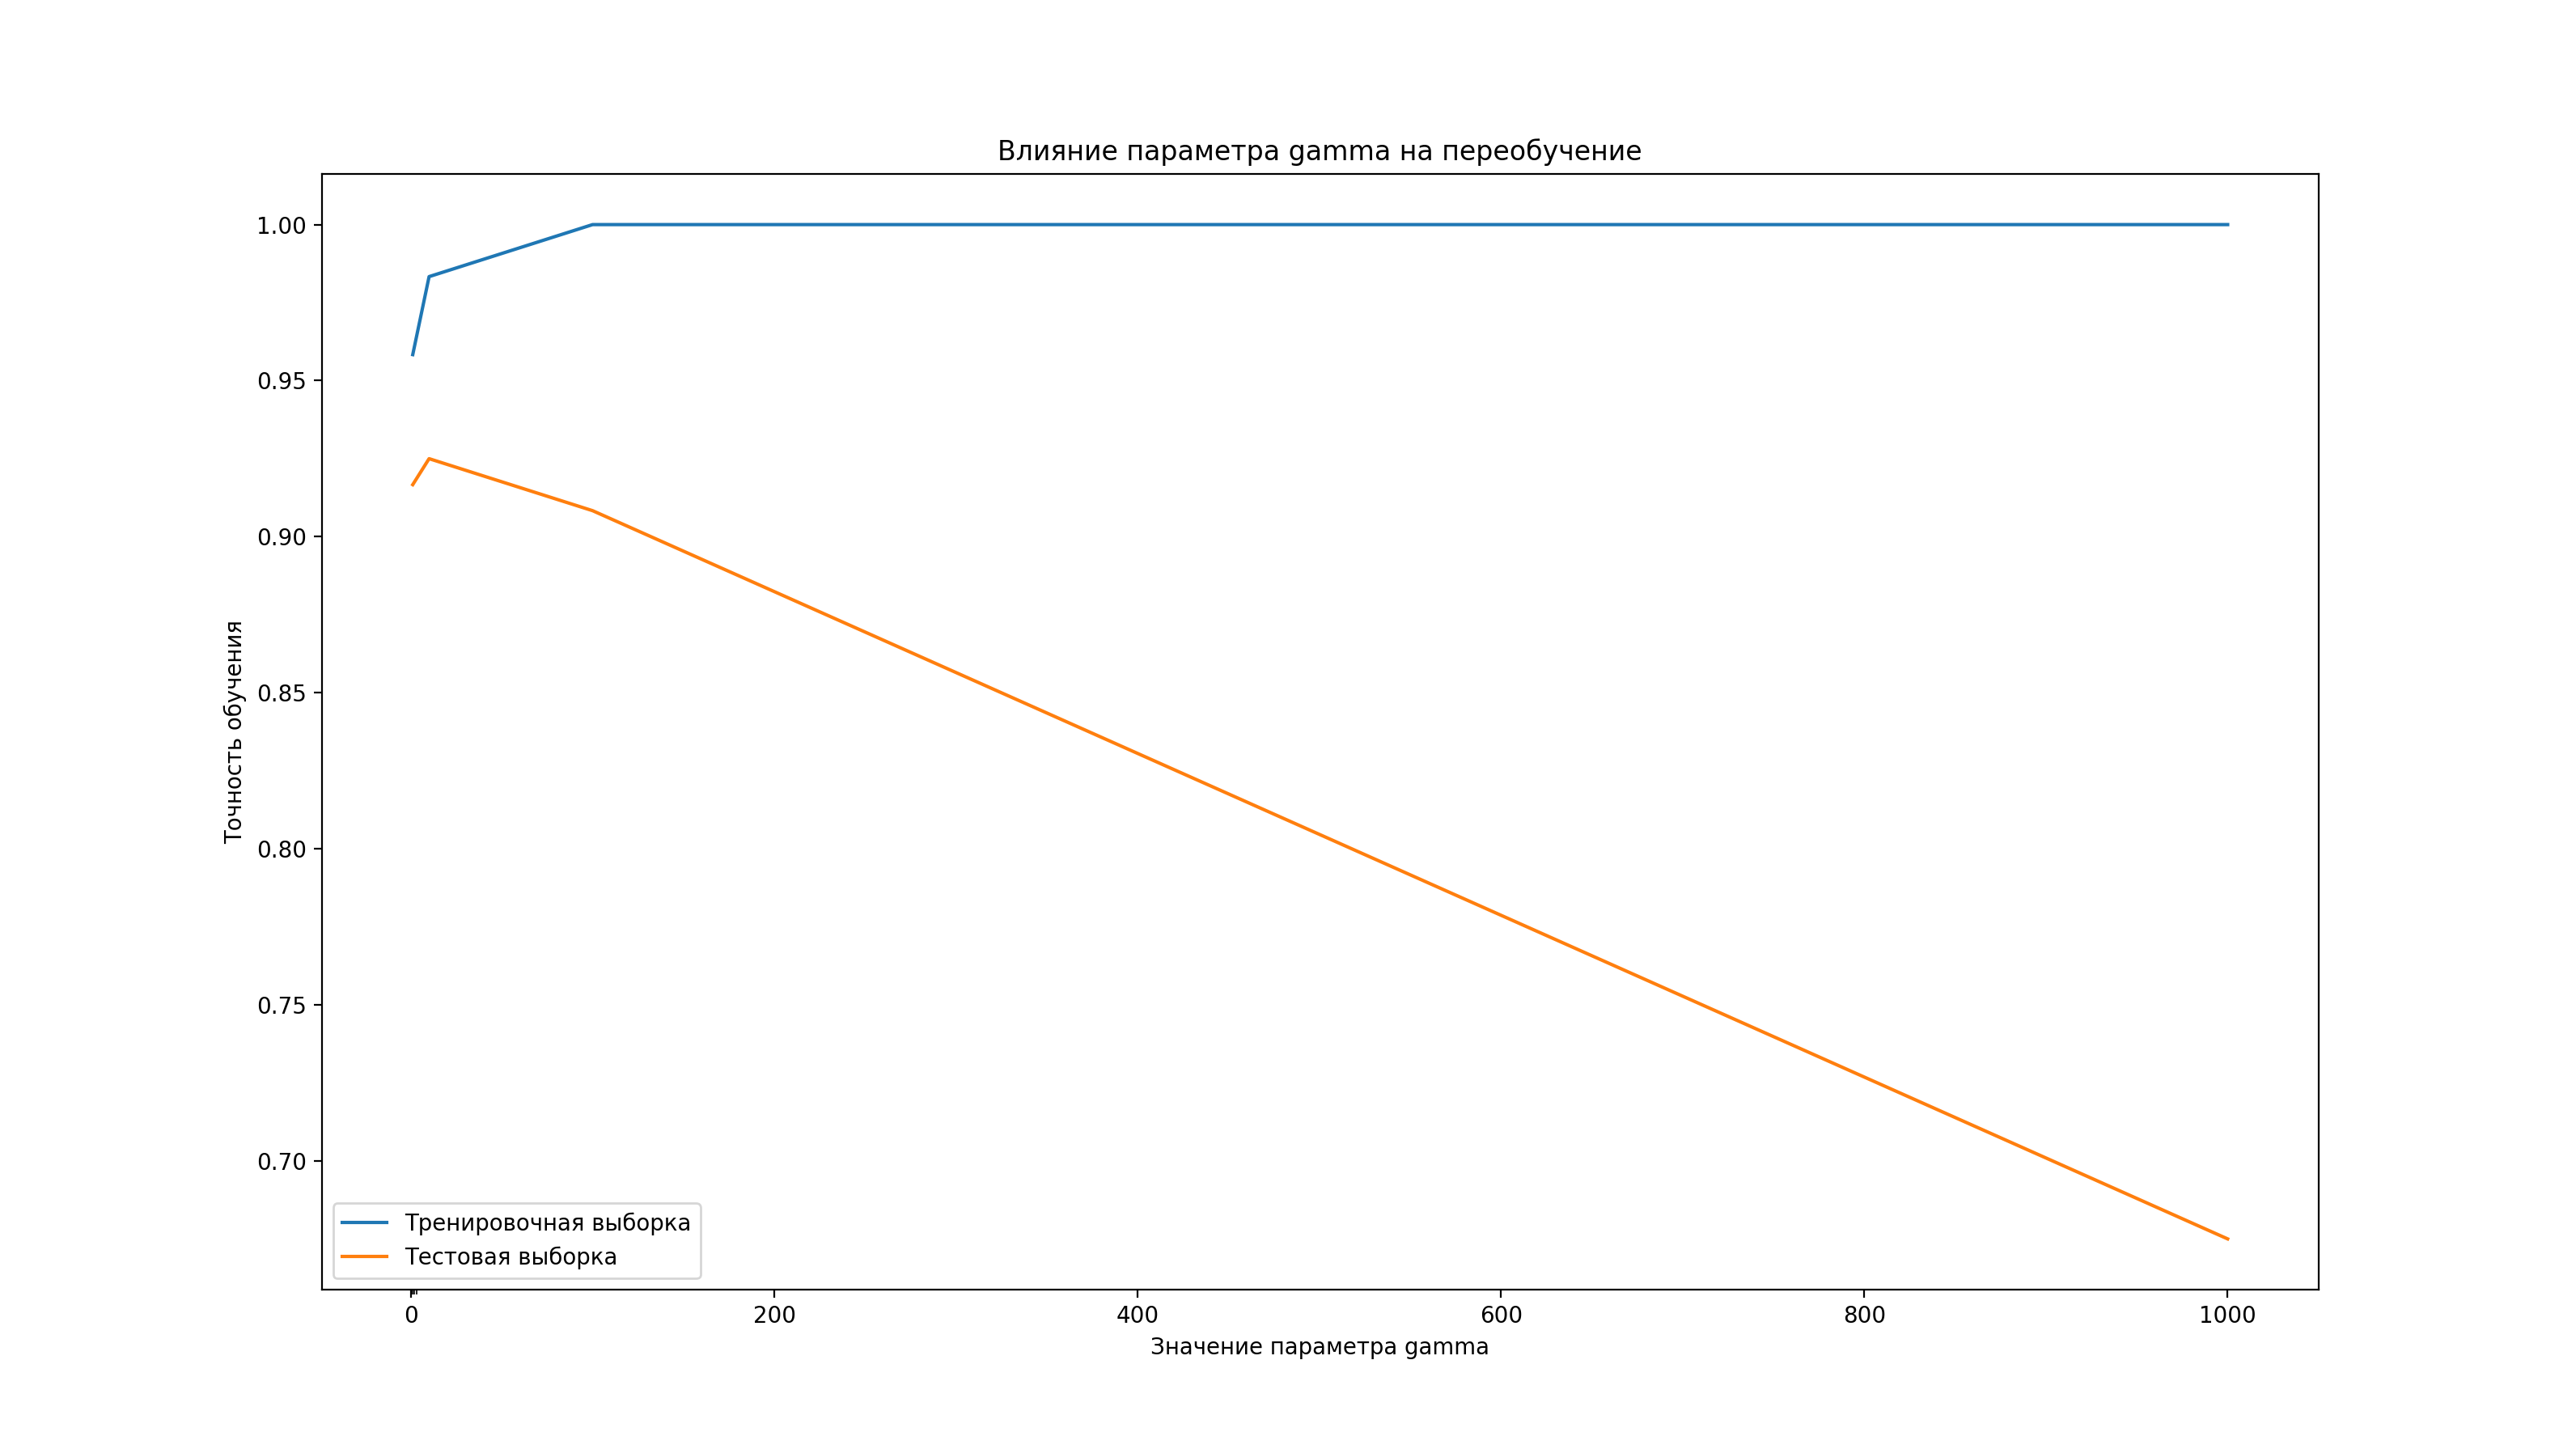
\includegraphics[width=\textwidth, keepaspectratio]{task5_gamma.png}
\caption{Переобучение на датасете 5}
\label{graph:task_5_gamma}
\end{figure}



\end{document}